
\let\negmedspace\undefined
\let\negthickspace\undefined
\documentclass[journal,12pt,twocolumn]{IEEEtran}
%\documentclass[conference]{IEEEtran}
%\IEEEoverridecommandlockouts
% The preceding line is only needed to identify funding in the first footnote. If that is unneeded, please comment it out.
\usepackage{cite}
\usepackage{amssymb,amsfonts,amsthm,amsmath}
\usepackage{algorithmic}
\usepackage{graphicx}
\usepackage{textcomp}
\usepackage{xcolor}
\usepackage{txfonts}
\usepackage{listings}
\usepackage{enumitem}
\usepackage{mathtools}
\usepackage{gensymb}
\usepackage{bm}

%%
%\usepackage{setspace}
%%\doublespacing
%\singlespacing
%
%%\usepackage{graphicx}
%%\usepackage{amssymb}
%%\usepackage{relsize}
%\usepackage[cmex10]{amsmath}
%%\interdisplaylinepenalty=2500
%%\savesymbol{iint}
%%\usepackage{txfonts}
%%\restoresymbol{TXF}{iint}
%%\usepackage{wasysym}
%\usepackage{amsthm}
%\usepackage{mathrsfs}
%\usepackage{txfonts}
%%\usepackage{stfloats}
%%\usepackage{cite}
%%\usepackage{cases}
%%\usepackage{subfig}
%%\usepackage{xtab}
%%\usepackage{multirow}
%%\usepackage{algorithm}
%%\usepackage{algpseudocode}
\usepackage{tikz}
%%\usepackage{circuitikz}
%%\usepackage{verbatim}
\usepackage{hyperref}
%%\usepackage{stmaryrd}
%%\usepackage{tkz-euclide} % loads  TikZ and tkz-base
%%\usetkzobj{all}
    \usepackage{color}                                            %%
    \usepackage{array}                                            %%
    \usepackage{longtable}                                        %%
    \usepackage{calc}                                             %%
    \usepackage{multirow}                                         %%
    \usepackage{hhline}                                           %%
    \usepackage{ifthen}                                           %%
%  %optionally (for landscape tables embedded in another document): %%
%    \usepackage{lscape}     
%%\usepackage{multicol}
%\usepackage{chngcntr}
%\usepackage{enumerate}

%\usepackage{wasysym}
%\newcounter{MYtempeqncnt}
\DeclareMathOperator*{\Res}{Res}
%\renewcommand{\baselinestretch}{2}
\renewcommand\thesection{\arabic{section}}
\renewcommand\thesubsection{\thesection.\arabic{subsection}}
\renewcommand\thesubsubsection{\thesubsection.\arabic{subsubsection}}

\renewcommand\thesectiondis{\arabic{section}}
\renewcommand\thesubsectiondis{\thesectiondis.\arabic{subsection}}
\renewcommand\thesubsubsectiondis{\thesubsectiondis.\arabic{subsubsection}}

% correct bad hyphenation here
\hyphenation{op-tical net-works semi-conduc-tor}
\def\inputGnumericTable{}                                 %%

\lstset{
language=tex,
frame=single, 
breaklines=true
}

\begin{document}
%


\newtheorem{theorem}{Theorem}[section]
\newtheorem{problem}{Problem}
\newtheorem{proposition}{Proposition}[section]
\newtheorem{lemma}{Lemma}[section]
\newtheorem{corollary}[theorem]{Corollary}
\newtheorem{example}{Example}[section]
\newtheorem{definition}[problem]{Definition}
%\newtheorem{thm}{Theorem}[section] 
%\newtheorem{defn}[thm]{Definition}
%\newtheorem{algorithm}{Algorithm}[section]
%\newtheorem{cor}{Corollary}
\newcommand{\BEQA}{\begin{eqnarray}}
\newcommand{\EEQA}{\end{eqnarray}}
\newcommand{\define}{\stackrel{\triangle}{=}}
\newcommand*\circled[1]{\tikz[baseline=(char.base)]{
    \node[shape=circle,draw,inner sep=2pt] (char) {#1};}}

\bibliographystyle{IEEEtran}
%\bibliographystyle{ieeetr}


\providecommand{\mbf}{\mathbf}
\providecommand{\pr}[1]{\ensuremath{\Pr\left(#1\right)}}
\providecommand{\re}[1]{\ensuremath{\text{Re}\left(#1\right)}}
\providecommand{\im}[1]{\ensuremath{\text{Im}\left(#1\right)}}
\providecommand{\qfunc}[1]{\ensuremath{Q\left(#1\right)}}
\providecommand{\sbrak}[1]{\ensuremath{{}\left[#1\right]}}
\providecommand{\lsbrak}[1]{\ensuremath{{}\left[#1\right.}}
\providecommand{\rsbrak}[1]{\ensuremath{{}\left.#1\right]}}
\providecommand{\brak}[1]{\ensuremath{\left(#1\right)}}
\providecommand{\lbrak}[1]{\ensuremath{\left(#1\right.}}
\providecommand{\rbrak}[1]{\ensuremath{\left.#1\right)}}
\providecommand{\cbrak}[1]{\ensuremath{\left\{#1\right\}}}
\providecommand{\lcbrak}[1]{\ensuremath{\left\{#1\right.}}
\providecommand{\rcbrak}[1]{\ensuremath{\left.#1\right\}}}
\theoremstyle{remark}
\newtheorem{rem}{Remark}
\newcommand{\sgn}{\mathop{\mathrm{sgn}}}
\providecommand{\abs}[1]{\left\vert#1\right\vert}
\providecommand{\res}[1]{\Res\displaylimits_{#1}} 
\providecommand{\norm}[1]{\left\lVert#1\right\rVert}
%\providecommand{\norm}[1]{\lVert#1\rVert}
\providecommand{\mtx}[1]{\mathbf{#1}}
\providecommand{\mean}[1]{E\left[ #1 \right]}
\providecommand{\fourier}{\overset{\mathcal{F}}{ \rightleftharpoons}}
%\providecommand{\hilbert}{\overset{\mathcal{H}}{ \rightleftharpoons}}
\providecommand{\system}{\overset{\mathcal{H}}{ \longleftrightarrow}}
	%\newcommand{\solution}[2]{\textbf{Solution:}{#1}}
\newcommand{\solution}{\noindent \textbf{Solution: }}
\newcommand{\cosec}{\,\text{cosec}\,}
\providecommand{\dec}[2]{\ensuremath{\overset{#1}{\underset{#2}{\gtrless}}}}
\newcommand{\myvec}[1]{\ensuremath{\begin{pmatrix}#1\end{pmatrix}}}
\newcommand{\mydet}[1]{\ensuremath{\begin{vmatrix}#1\end{vmatrix}}}
	\newcommand*{\permcomb}[4][0mu]{{{}^{#3}\mkern#1#2_{#4}}}
\newcommand*{\perm}[1][-3mu]{\permcomb[#1]{P}}
\newcommand*{\comb}[1][-1mu]{\permcomb[#1]{C}}

%\numberwithin{equation}{section}
\numberwithin{equation}{subsection}
%\numberwithin{problem}{section}
%\numberwithin{definition}{section}
\makeatletter
\@addtoreset{figure}{problem}
\makeatother

\let\StandardTheFigure\thefigure
\let\vec\mathbf
\let\j\jmath
%\renewcommand{\thefigure}{\theproblem.\arabic{figure}}
\renewcommand{\thefigure}{\theproblem}
%\setlist[enumerate,1]{before=\renewcommand\theequation{\theenumi.\arabic{equation}}
%\counterwithin{equation}{enumi}


%\renewcommand{\theequation}{\arabic{subsection}.\arabic{equation}}

\def\putbox#1#2#3{\makebox[0in][l]{\makebox[#1][l]{}\raisebox{\baselineskip}[0in][0in]{\raisebox{#2}[0in][0in]{#3}}}}
     \def\rightbox#1{\makebox[0in][r]{#1}}
     \def\centbox#1{\makebox[0in]{#1}}
     \def\topbox#1{\raisebox{-\baselineskip}[0in][0in]{#1}}
     \def\midbox#1{\raisebox{-0.5\baselineskip}[0in][0in]{#1}}

\vspace{3cm}




\title{CBSE MATHEMATICS 2020}
\author{G V V Sharma$^{*}$
	\thanks{}
}
% make the title area
\maketitle

\newpage

\tableofcontents

\bigskip

\renewcommand{\thefigure}{\theenumi}
\renewcommand{\thetable}{\theenumi}
\renewcommand{\theequation}{\theenumi}

\section{Matrices}
\begin{enumerate}[label=\thesection.\arabic*.,ref=\thesection.\theenumi]
\numberwithin{equation}{enumi}
\numberwithin{figure}{enumi}
\numberwithin{table}{enumi}
\item Show that the plane $ x-5y-2z=1 $ contains the line $ \frac{x-5}{3}=y=2-z $ .\\
	\solution The plane and line can be expressed in vector form as
  \begin{align}
	  \label{eq:line_plane_contain_plane}
	  \myvec{1 & -5 & -2}\vec{x}=1 
	  \\
	  \vec{x} = \myvec{5 \\ 0 \\ 2} + \lambda \myvec{3 \\ 1 \\ -1}
	  \label{eq:line_plane_containline}
  \end{align}
The plane contains the line if 
  \begin{align}
	  \vec{m}^{\top}\vec{n} = 0
  \end{align}
  The input parameters are 
  \begin{align}
	  \vec{m} = \myvec{3 \\ 1 \\ -1},
	 \vec{n} = \myvec{1 & -5 & -2}.
  \end{align}
  $\because$
  \begin{align}
	  \myvec{1 & -5 & -2}\myvec{3 \\ 1 \\ -1} = 0,
	  \label{eq:line_plane_containline_sol}
  \end{align}
the given plane contains the given line.
\item  Find a vector $\overrightarrow{r}$ equally inclined to the three axes and whose magnitude is $3\sqrt{3}$ units.   
	\\
	\solution  Let $\vec{e}_1, \vec{e}_2, \vec{e}_3$ be the standard basis vectors (direction vectors of the coordinate axes) such that
  \begin{align}
	  \myvec{\vec{e}_1 & \vec{e}_2 &\vec{e}_3} = \vec{I}
  \end{align}
  Then, 
  \begin{align}
	  \frac{\vec{e}_1^{\top} \vec{r}}{\norm{\vec{e}_1}\norm{\vec{r}}} = 
	  \frac{\vec{e}_2^{\top} \vec{r}}{\norm{\vec{e}_2}\norm{\vec{r}}} = 
	  \frac{\vec{e}_3^{\top} \vec{r}}{\norm{\vec{e}_3}\norm{\vec{r}}} = \cos \theta
  \end{align}
  which can be expressed as the system of equations
  \begin{align}
	  {\vec{e}_1^{\top} \vec{r}} = \norm{\vec{r}}\cos \theta
	  \\
	  {\vec{e}_2^{\top} \vec{r}} = \norm{\vec{r}}\cos \theta
	  \\
	  {\vec{e}_3^{\top} \vec{r}} = \norm{\vec{r}}\cos \theta
  \end{align}
  which can be combined to obtain the matrix equation
  \begin{align}
	  \myvec{\vec{e}_1 & \vec{e}_2 & \vec{e}_3}^{\top}\vec{r} &= \norm{\vec{r}}\cos \theta \myvec{1\\1\\1}
	  \\
	  \implies \frac{\vec{r}}{\norm{\vec{r}}}&= \cos \theta \myvec{1\\1\\1}
	  \label{eq:equal_incline_unit}
  \end{align}
  \begin{align}
	  \because 	\myvec{\vec{e}_1 & \vec{e}_2 & \vec{e}_3} = \vec{I}
  \end{align}
  From 
	  \eqref{eq:equal_incline_unit}
  \begin{align}
	  \norm {\cos \theta \myvec{1\\1\\1}} &= 1
	  \\
	  \implies\cos \theta  = \frac{1}{\sqrt{3}}
	  \label{eq:equal_incline_unit_cos}
  \end{align}
 From  
	  \eqref{eq:equal_incline_unit_cos} and 
	  \eqref{eq:equal_incline_unit}

  \begin{align}
	  \vec{r} &=  3\sqrt{3}\times \frac{1}{\sqrt{3}}\myvec{1\\1\\1}
	  \\
		  &=3\myvec{1\\1\\1}
	  \label{eq:equal_incline_unit_ans}
  \end{align}
\item Find the angle between unit vectors $\overrightarrow{a}$ and $\overrightarrow{b}$ so that $\sqrt{3}$ $\overrightarrow{a}$ - $\overrightarrow{b}$ is also a unit vector.\\
	\solution 
	From the given information, the coordinate vector  is 
  \begin{align}
	  \vec{x} = \myvec{\sqrt{3} \\ -1}
			\label{eq:misc-x}
  \end{align}
  The angle between the vectors is then given by 
		\begin{align}
	\cos \theta
			= \frac{1 - \norm{\vec{x}}^2}{\vec{x}^{\top}\vec{R}\vec{x}}
			\label{eq:misc-c-ellipse-d-rho-final}
		\end{align}
		where 
		\begin{align}
			\vec{R}	&= \myvec{0 & 1 \\ 1 & 0}.
		\end{align}
		By substituting from 
			\eqref{eq:misc-x}
			in 
			\eqref{eq:misc-c-ellipse-d-rho-final}
  \begin{align}
\cos \theta=   \frac{\sqrt{3}}{2} \implies \theta = 30 \degree
  \end{align}
\item If $\vec{A}=\myvec{-3 & 2 \\ 1 & -1} $ and $ \vec{I}=\myvec{1 & 0 \\ 0 & 1}$, Find scalar k so that $\vec{A}^2 + \vec{I} = k\vec{A}$.\\
	\solution Using the Cayley-Hamilton theorem, 
  \begin{align}
	  \lambda^2 - k \lambda + 1 = 0
	  \label{eq:cayley_applic}
  \end{align}
  Since the trace of the matrix is equal to the sum of its eigenvalues, 
  \begin{align}
	   k  = \lambda_1+\lambda_2 = \text{tr}\brak{\vec{A}} = -3-1 = -4
	  \label{eq:cayley_sol}
  \end{align}
\item  Find the coordinates of the point where the line 
        \begin{align}
        \frac{x-1}{3} = \frac{y+4}{7} = \frac{z+4}{2}
        \nonumber
	\end{align} 
        cuts the xy-plane. \\
	\solution 
	The given line can be expressed as 
	\begin{align}
		\vec{x} = \myvec{1 \\ -4 \\ -4} + \lambda \myvec{3 \\ 7 \\ 2}
		\label{eq:cbse_12_line_plane}
\end{align}
and the $xy$- plane is 
	\begin{align}
		\myvec{0 & 0 &1}\vec{x}  = 0
		\label{eq:cbse_12_line_plane_eq}
\end{align}
The desired point can be obtained as 
\begin{align}
		\label{eq:cbse_12_line_plane_eq-isect}
	\vec{x} &= \vec{A} + \frac{c - \vec{n}^{\top}\vec{A}}{\vec{n}^{\top}\vec{m}}
\vec{m}
\end{align}
Substiuting the input parameters
\begin{align}
	\vec{m} = \myvec{3 \\ 7 \\ 2},
	\vec{A} = \myvec{1 \\ -4 \\ -4},
	\vec{n} = \myvec{0 & 0 &1},
	\vec{c} = 0,
\end{align}
		in \eqref{eq:cbse_12_line_plane_eq-isect},
\begin{align}
	& \myvec{1 \\ -4 \\ -4} + \frac{0 - \myvec{0 & 0 &1}\myvec{1 \\ -4 \\ -4}}{\myvec{0 & 0 &1}\myvec{3 \\ 7 \\ 2}}\myvec{3 \\ 7 \\ 2}
	\\
	&=\myvec{1 \\ -4 \\ -4}+2\myvec{3 \\ 7 \\ 2}
	\\
	&=\myvec{7 \\ 10 \\ 0}
\end{align}
\item  The angle between the vectors $ \hat{i} - \hat{j} $ and $ \hat{j} - \hat{k} $ is

\begin{enumerate}
    \item $\frac{-\pi}{3}$
    \item 0
    \item $\frac{\pi}{3}$
    \item $\frac{2\pi}{3}$
\end{enumerate}
\solution 
The angle between the vectors $\vec{m}_1, \vec{m}_2$ is given by 
  \begin{align}
	  \label{eq:matrix-ang-vec}
	  \cos \theta = \frac{\vec{m}_1^{\top} \vec{m}_2}{\norm{\vec{m}_1}\norm{ \vec{m}_2}}
  \end{align}
  Substituting 
  \begin{align}
\vec{m}_1 = \myvec{1 \\ -1 \\ 0}, \vec{m}_2 = \myvec{0 \\ 1 \\ -1}
  \end{align}
	  in \eqref{eq:matrix-ang-vec},
%
  \begin{align}
	  \myvec{1 & -1 & 0} \myvec{0 \\ 1 \\ -1} &= -1,
	  \\
	  \norm{\myvec{1 \\ -1 \\ 0}}=\norm{\myvec{0 \\ 1 \\ -1}} &= \sqrt{2}
	  \\
	  \implies \cos \theta &= \frac{-1}{2}
	  \\
	  \text{or, }\theta &= \frac{2\pi}{3}
  \end{align}

\item  If $\vec{A}$ is a non-singular square matrix of order 3 such that $ \vec{A}^2 =3\vec{A} $, then value of  $\begin{vmatrix}\vec{A} \end{vmatrix}$ is

\begin{enumerate}
    \item -3
     \item 3
     \item 9
     \item 27
\end{enumerate}
  \begin{align}
	  \mydet {\vec{A}^2} &=\mydet{3\vec{ A}}
	  \\
	  \implies 
	  \mydet {\vec{A}} ^2&=3^3\mydet{\vec{ A}}
  \end{align}
	yielding 
  \begin{align}
	  \mydet {\vec{A}} &=27
  \end{align}
  after simplification.
\item  If $\mydet{\overrightarrow{a}} = 4 $ and  $ -3\leq \lambda \leq 2 $ then $\mydet{\lambda \overrightarrow{a}} $ lies in

\begin{enumerate}
    \item $\left[0,12\right]$
    \item $\left[2,3\right]$
    \item $\left[8,12\right]$
    \item $\left[-12,8\right]$
\end{enumerate}
	 \solution  
\begin{align}
  \norm{\lambda \vec{a}} 
  &= \abs{\lambda} \norm{\vec{a}}
  \\
	&= 4\abs{\lambda} 
\end{align}
$\because$
\begin{align}
	0 \leq \abs{\lambda} \leq 3,  
\\
	0 \leq 4\abs{\lambda} \leq 12
\end{align}
\item The area of a triangle formed by vertices O, A and B, where $\overrightarrow{OA}=\hat{i} + 2\hat{j} + 3 \hat{k} $ and $\overrightarrow{OB}=-3\hat{i} - 2\hat{j} +  \hat{k} $ is \\
 \begin{enumerate}
     \item $ 3\sqrt{5} $ sq.units\\
    \item$ 5\sqrt{5} $ sq.units\\
    \item$ 6\sqrt{5} $ sq.units\\
    \item$ 4 $ sq.units
\end{enumerate}
\solution Let
		\begin{align}
			\vec{A} = \myvec{1 \\ 2 \\ 3},
			\vec{B}  = \myvec{-3 \\ -2 \\ 1},
		\end{align}
In general, the area of $\triangle OAB$ can be expressed as
		\begin{align}
		\frac{1}{2}	\norm{\brak{\vec{A}-\vec{O}}  \times 
			\brak{\vec{B}- \vec{O}}}  
		\end{align}
$\because $
		\begin{align}
			\myvec{2 & -2 \\ 3 & 1 } &= 8,
\\
			\myvec{3 & 1 \\ 1 & -3 } &= -10,
			\\
			\myvec{1 & -3 \\ 2 & -2 } &= 4,
		\end{align}
		\begin{align}
			\vec{A}  \times 
			\vec{B}  = \myvec{8 \\ -10 \\ 4},
		\end{align}
		and the  desired area can be obtained as 
		\begin{align}
			\frac{1}{2}\norm{\myvec{8 \\ -10 \\ 4}} = 3 \sqrt{5}
		\end{align}
\item  The coordinates of the foot of the perpendicular drawn from the point $ \left(2,-3,4 \right) $ on the $y$-axis is 

\begin{enumerate}
    \item $\left(2,3,4\right)$
    \item $\left(-2,-3,-4\right)$
    \item $\left(0,-3,0\right)$
    \item $\left(2,0,4\right)$
\end{enumerate}
\solution 
In general, let $\vec{P}$ be any point and the line be
\begin{align}
	\label{cbse_12_foot_perp_line}
	L: \quad	\vec{x} &=  \vec{A} + \lambda \vec{m}
		\end{align}
\begin{align}
	\label{cbse_12_foot_perp_pt}
\vec{x} &=  \vec{A} + \frac{	\vec{m}^{\top}\brak{\vec{P}  -  \vec{A}}}{\norm{\vec{m}}^2}\vec{m}
		\end{align}
The equation of the $y$-axis can be written as	
		\begin{align}
			\vec{x} = \lambda 	\myvec{0 \\ 1 \\ 0} 
		\end{align}
		Substituting the input parameters 
		\begin{align}
			\vec{P} =  	\myvec{2 \\ -3 \\ 4},  
			\vec{A} =  	\myvec{0 \\ 0 \\ 0},  
			\vec{m} =  	\myvec{0 \\ 1 \\ 0},  
		\end{align}
	in \eqref{cbse_12_foot_perp_pt},
  the desired point is given by 
\begin{align}
	\vec{x} &=   \myvec{0 & 1 & 0}\myvec{2 \\-3 \\4 } 
 \myvec{0 \\ 1 \\ 0} 
 \\
	&=
 \myvec{0 \\ -3 \\ 0} 
		\end{align}
\item  The distance between parallel planes 2x+y-2z-6=0 and 4x+2y-4z=0 is ------------------ units.
	\\
\solution The above planes have parameters
	\begin{align}
		\vec{n} = \myvec{2 & 1 & -2}, c_1=6, c_2 = 0
\end{align}
The distance is then obtained as

\begin{align}
	d &= \frac{\abs{c_1-c_2}}{\norm{\vec{n}}} 
\\
	&= \frac{6}{3} = 2
\end{align}

\item If P(1,0,-3) is the foot of the perpendicular from the origin to the plane, then the Cartesian equation of the plane is .................... \\
    \solution Let the equation of the plane be 
	\begin{align}
		\vec{n}^{\top}\vec{x} = c
\end{align}
Since $\vec{P}$ is a point on the plane, it satisfies the above equation and 
	\begin{align}
		\vec{n}^{\top}\vec{P} = c
		\label{eq:cbse_12_foot}
\end{align}
The normal vector to the plane is $OP$.  Hence, 
	\begin{align}
		\vec{n} = \vec{P} 
\end{align}
		Substituting the above in \eqref{eq:cbse_12_foot},
	\begin{align}
		\vec{P}^{\top}\vec{P} = c
		\label{eq:cbse_12_foot_sub}
\end{align}
and the desired equation of the plane is 
	\begin{align}
		\vec{P}^{\top}\vec{x} &= 		\vec{P}^{\top}\vec{P}
		\\
		\myvec{1 & 0 &-3}\vec{x} &= 	10	
		\label{eq:cbse_12_foot_ans}
\end{align}
   after substituting numerical values. 
    
\item Find the equation of the plane passing through the points $(1,0,-2)$ , $(3,-1,0)$ and perpendicular to the plane $ 2x-y+z=8 $. Also find the distance of the plane thus obtained from the origin.\\
\solution Let the equation of the desired plane be 
\begin{align}
	\vec{n}^{\top}\vec{x} = 1
%	\\
%	\myvec{1 \\0 \\-2} \myvec{3 \\ -1 \\0}
  \end{align}
  From the given information, 
\begin{align}
	\vec{n}^{\top}\vec{x} &= 1
	\\
\implies
\begin{split}
	\myvec{1 &0 &-2} \vec{n} &=1 
	\\
	\myvec{3 & -1 &0}\vec{n} &=1
	\\
	\myvec{2 & -1 & 1}\vec{n} &=0
	\end{split}
	\label{eq:plane_pt_perp}
  \end{align}
From 
	\eqref{eq:plane_pt_perp},
	we obtain  the matrix equation
\begin{align}
	\myvec{1 &0 &-2\\ 3 & -1 &0 \\ 2 & -1 & 1} \vec{n} &= \myvec{1 \\ 1 \\ 0}
  \end{align}
Forming the augmented matrix, and choosing the pivot,
\begin{align}
	\myvec{\circled{1} &0 &-2 & \vrule &  1\\ 3 & -1 &0 & \vrule &1\\ 2 & -1 & 1 & \vrule &0} 
	\\
	\xleftrightarrow[]{}
	\myvec{1 &0 &-2 & \vrule &  1\\ 0 & \circled{1} &-6 & \vrule &2\\ 0 & -1 & 5 & \vrule &-2} 
	\\
	\myvec{1 &0 &-2 & \vrule &  1\\ 0 & 1 &-6 & \vrule &2\\ 0 & 0 & \circled{1} & \vrule &0} 
  \end{align}
  yielding 
\begin{align}
\vec{n} =\myvec{1 \\ 2 \\ 0} 
  \end{align}
  Thus, the equation of the desired plane is 
\begin{align}
\myvec{1 & 2 & 0} \vec{n} = 1
  \end{align}
\item  If \begin{align} \mydet{2x & -9 \\ -2 & x}  = \mydet{-4 & 8 \\ 1 & -2 } \nonumber \end{align} then value of x is -------------\\
\solution
		Expanding the above determinants,
\begin{align}
	2x^2 - 18 &= 0
	\\
	\implies x &= \pm 3
\end{align}
 \item Using integration, find the area lying above x-axis and included between the circle $ x^2 + y^2 =8x $ and inside the parabola $ y^2 =4x $.   
	 \\
	 \solution The given circle and parabola can be expressed as conics with parameters
\begin{align}
	\vec{V}_1 &= \vec{I}, \vec{u}_1 = -\myvec{4 \\0}, f_1 = 0
	\\
	\vec{V}_2 &= \myvec{ 0 & 0 \\ 0 & 1}, \vec{u}_2 = -\myvec{2 \\0}, f_2 = 0
    \end{align}
    The intersection of the given conics is obtained as 
\begin{align}
	\vec{x}^{\top}\brak{\vec{V}_1 + \mu\vec{V}_2}\vec{x}+2 \brak{\vec{u}_1+\mu \vec{u}_2}^{\top} \vec{x} 
	\\
	+ \brak{f_1+\mu f_2}= 0
    \end{align}
    This conic is a pair of straight lines if  and only if 
\begin{align}
	\mydet{\vec{V}_1 + \mu\vec{V}_2 & \vec{u}_1+\mu \vec{u}_2\\ \brak{\vec{u}_1+\mu \vec{u}_2}^{\top} & f_1 + \mu f_2} &= 0
	\\
	\label{eq:conic-pair}
	\mydet{\vec{V}_1 + \mu\vec{V}_2} &< 0
\\
	\implies 	\mydet{1 & 0 & -4-2\mu\\ 0 & 1+\mu & 0 \\ -4 - 2\mu & 0 & 0} &= 0
    \end{align}
    upon substituting numerical values, which can be expanded to obtain 
\begin{align}
	\brak{\mu + 1}\brak{\mu + 2}^2 &= 0
    \end{align}
    yielding
\begin{align}
\mu =  -2
    \end{align}
upon checking for \eqref{eq:conic-pair}.  Thus, the parameters for the pair of straight lines can be expressed as
\begin{align}
	\vec{V} &= 
\vec{V}_1 + \mu\vec{V}_2
=\myvec{ 1 & 0 \\ 0 & -1},
\\
	\vec{u} &=
\vec{u}_1+\mu \vec{u}_2
	= \vec{0},
\\
	f&=0,
	\\
	\implies \vec{D} &= \vec{V}, \vec{P} = \vec{I}
\label{eq:quad_form_pair-param}
    \end{align}
    Thus, the desired pair of straight lines are 
\begin{align} 
	\myvec{\sqrt{\abs{\lambda_1}} & \pm \sqrt{\abs{\lambda_2}}}\vec{P}^{\top}\brak{\vec{x}-\vec{c}} &= 0
	\\
	\implies 
	\myvec{1 & \pm 1}\vec{x} &= 0
	\\
	\text{or, }\vec{x} &= \kappa \myvec{\pm 1 \\ 1}
\end{align} 
upon substituting from 
\eqref{eq:quad_form_pair-param}.
The points of intersection of the line 
\begin{align}
L: \quad \vec{x} = \vec{q} + \kappa \vec{m} \quad \kappa \in \mathbb{R}
\label{eq:conic_tangent}
\end{align}
with the conic section 
\begin{align}
	\vec{x}^{\top}\vec{V}\vec{x} + 2\vec{u}^{\top} \vec{x} + f = 0
\label{eq:conic_quad_form}
\end{align}
are given by
\begin{align}
\vec{x}_i = \vec{q} + \kappa_i \vec{m}
\label{eq:conic_tangent_pts}
\end{align}
%
where
{\tiny
\begin{multline}
\kappa_i = \frac{1}
{
\vec{m}^T\vec{V}\vec{m}
}
\lbrak{-\vec{m}^T\brak{\vec{V}\vec{q}+\vec{u}}}
\\
\pm
\rbrak{\sqrt{
\sbrak{
\vec{m}^T\brak{\vec{V}\vec{q}+\vec{u}}
}^2
-
\brak
{
\vec{q}^T\vec{V}\vec{q} + 2\vec{u}^T\vec{q} +f
}
\brak{\vec{m}^T\vec{V}\vec{m}}
}
}
\label{eq:tangent_roots}
\end{multline}
}
Substituting
\begin{align}
	\vec{q} &= \vec{0}, \vec{m} = \myvec{1 \\ 1}
	\\
	\vec{V} &= \vec{I},
	\vec{u} = -\myvec{4 \\0}
	f = 0
\end{align}
in 
\eqref{eq:tangent_roots}, the intersection parameters $\kappa_i$ of the line 
\begin{align}
	\myvec{1 & - 1}\vec{x} &= 0
\end{align}
with the given circle are
\begin{align}
\kappa = 0, 4 
\end{align}
and the points of intersection are 
\begin{align}
	\vec{0}, \myvec{4 \\ 4}
\end{align}
Similarly, 
the points of intersection of the line 
\begin{align}
	\myvec{1 & - 1}\vec{x} &= 0
\end{align}
with the given circle are 
\begin{align}
	\vec{0}, \myvec{4 \\ -4}
\end{align}
%
Thus the intersection of the parabola with the circle above the $x$-axis are the points 
\begin{align}
	\vec{0}, \myvec{4 \\ 4}
\end{align}
From Fig. 
	\ref{fig:matrix-12-15},
\begin{figure}[!ht]
	\centering
	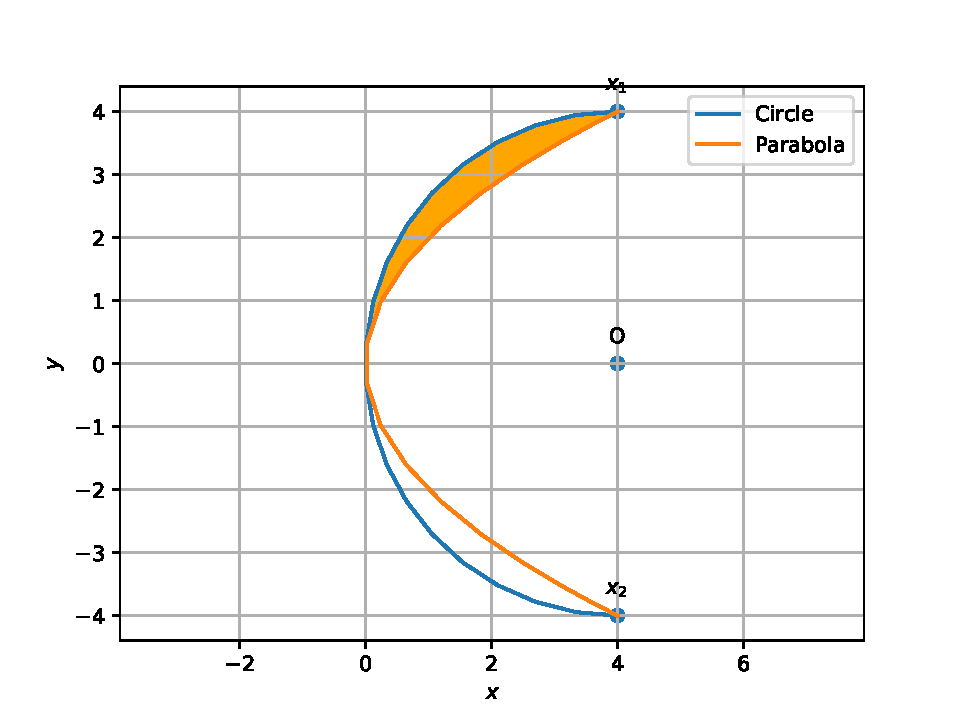
\includegraphics[width=\columnwidth]{figs/matrix-12-15.pdf}
	\caption{}
	\label{fig:matrix-12-15}
\end{figure}
the area covered by the parabola is given by 
\begin{align}
	\int_{0}^{4}2\sqrt{x} &= \frac{4}{3}\sbrak{x^{\frac{3}{2}}}_{0}^4{}	
	\\
	&= \frac{32}{3}
\end{align}
The area covered by the circle is
\begin{align}
	\frac{\pi r^2}{4} = 4\pi
\end{align}
Thus, the desired area is 
the shaded region in Fig. 
	\ref{fig:matrix-12-15},
	and given by 
\begin{align}
 4\pi - \frac{32}{3}
\end{align}





    
\item Using the method of integration, find the area of the triangle ABC, coordinates of whose vertices are A(2,0), B(4,5) and C(6,3).\\
    \solution Since 
\begin{align}
	\vec{A}-\vec{B} &= \myvec{-2 \\-5},
	\\
	\vec{A}-\vec{C} &= \myvec{-4 \\-3},
    \end{align}
    the desired area is  the magnitude of 
\begin{align}
 \mydet{2 & 4\\5 & 3} 
    \end{align}
    Thus the desired area is 14 units.
\item If $A=\myvec{5 & -1 & 4 \\ 2 & 3 & 5 \\ 5 & -2 & 6} $, Find $A^{-1}$ and use it to solve the following system of the equations: \\
\begin{align}
	5x-y+4z &= 5 \nonumber \\
	2x+3y+5z &= 2 \nonumber \\
	5x-2y+6z &= -1 
\nonumber
\end{align}
   \solution Forming the augmented matrix and pivoting,  
\begin{align}
	\myvec{\circled{5} & -1 & 4 & \vrule & 1 & 0 & 0\\ 2 & 3 & 5 & \vrule & 0 & 1 & 0\\ 5 & -2 & 6 & \vrule & 0 & 0 & 1}
	\\
	\xleftrightarrow []{}
	\myvec{5 & -1 & 4 & \vrule & 1 & 0 & 0\\ 0 & \circled{17} & 17 & \vrule & -2 & 5 & 0\\ 0 & 1 & -2 & \vrule & 1 & 0 & -1}
	\\
	\xleftrightarrow []{}
	\myvec{17 & 0 & 17 & \vrule & 3 & 1 & 0\\ 0 & 17 & 17 & \vrule & -2 & 5 & 0\\ 0 & 0 & \circled{51} & \vrule & -19 & 5 & 17}
	\\
	\xleftrightarrow [R_2\leftarrow 3R_2 - R_3]{R_1\leftarrow 3R_1 - R_3}
	\\
	\myvec{51 & 0 & 0 & \vrule & 28 & -2& -17\\ 0 & 51 & 0 & \vrule & 13 & 10 & -17\\ 0 & 0 & 51 & \vrule & -19 & 5 & 17}
    \end{align}
    resulting in 
\begin{align}
	\vec{A}^{-1} = \frac{1}{51}\myvec{ 28 & -2 & -17\\  13 & 10 & -17\\  -19 & 5 & 17}
    \end{align}
    Thus, letting 
\begin{align}
	\vec{b} &= \myvec{ 5 \\ 2 \\ -1},
	\\
	\vec{x} &= \vec{A}^{-1}\vec{b} = \frac{1}{51}\myvec{ 28 & -2 & -17\\  13 & 10 & -17\\  -19 & 5 & 17}\myvec{ 5 \\ 2 \\ -1}
	\\
	&= \myvec{ 3 \\ 2 \\ -2}
    \end{align}
    is the desired solution.
    
\item If x,y,z are different and 
\begin{align}
	\mydet{x & x^2 & 1+x^3 \\ y & y^2 & 1+y^3 \\ z & z^2 & 1+z^3 } =0 
	\label{eq:det_xyz_given}
    \end{align}

		then using properties of determinants show that \begin{align} 1+xyz=0 \nonumber \end{align}
	\solution The given determinant can be expressed as 
\begin{align}
	\mydet{x & x^2 & 1 \\ y & y^2 & 1 \\ z & z^2 & 1}  
	+\mydet{x & x^2 & x^3 \\ y & y^2 & y^3 \\ z & z^2 & z^3}  
	\label{eq:det_xyz}
%\xleftrightarrow[R_2 \leftarrow R_1 -R_2]{R_3 \leftarrow R_1 -R_3}
    \end{align}
    Since
\begin{align}
	\mydet{x & x^2 & x^3 \\ y & y^2 & y^3 \\ z & z^2 & z^3} 
	= xyz  
	\mydet{1 & x & x^2 \\ 1 & y & y^2 \\ 1 & z & z^2}  
	\label{eq:det_xyz_2}
%\xleftrightarrow[R_2 \leftarrow R_1 -R_2]{R_3 \leftarrow R_1 -R_3}
    \end{align}
    and 
\begin{align}
	\mydet{x & x^2 & 1 \\ y & y^2 & 1 \\ z & z^2 & 1} 
	= 
	\mydet{1 & x & x^2 \\ 1 & y & y^2 \\ 1 & z & z^2}, 
	\label{eq:det_xyz_12}
%\xleftrightarrow[R_2 \leftarrow R_1 -R_2]{R_3 \leftarrow R_1 -R_3}
    \end{align}
	\eqref{eq:det_xyz} can be expressed as
\begin{align}
	\brak{1+xyz}
	\mydet{1 & x & x^2 \\ 1 & y & y^2 \\ 1 & z & z^2}, 
	\label{eq:det_xyz_onefac}
    \end{align}
    The above determinant can be simplified as
\begin{align}
	\mydet{1 & x & x^2 \\ 1 & y & y^2 \\ 1 & z & z^2}, 
	\\
\xleftrightarrow[R_2 \leftarrow R_1 -R_2]{R_3 \leftarrow R_1 -R_3}
	\mydet{1 & x & x^2 \\ 0 & x-y & x^2-y^2 \\ 0 & x-z & x^2-z^2}, 
	\\
	=
	\brak{x-y}	\brak{x-z}\mydet{1 & x & x^2 \\ 0 & 1 & x+y \\ 0 & 1 & x+z}, 
	\\
	=
	\brak{x-y}\brak{y-z}	\brak{z-x}
    \end{align}
	and \eqref{eq:det_xyz_given} can be obtained from 
	\eqref{eq:det_xyz_onefac} as
\begin{align}
	\brak{1+xyz}
	\brak{x-y}\brak{y-z}	\brak{z-x} = 0
    \end{align}
    Since 
\begin{align}
	x \ne y \ne z, 
	\brak{1+xyz} = 0
    \end{align}
\end{enumerate}

\section{Continuous Math}
%\renewcommand{\theequation}{\theenumi}
\begin{enumerate}[label=\thesection.\arabic*.,ref=\thesection.\theenumi]
\numberwithin{equation}{enumi}
\numberwithin{figure}{enumi}
\numberwithin{table}{enumi}
 \item Evaluate : \begin{align} \int_{0}^{\frac{\pi}{2}} \sin2x \tan^{-1}  \left(\sin x\right)dx \nonumber \end{align}
		 \solution Let 
		 \begin{align}
			 \label{eq:cont_def_int_1}
			 \tan \theta = \sin x
		 \end{align}
		 Then 
		 \begin{align}
			 \label{eq:cont_def_int_2}
			 \sec^2  \theta \, d\theta= \cos x \, dx
		 \end{align}
			 From \eqref{eq:cont_def_int_1} and 
			 \eqref{eq:cont_def_int_2}
 \begin{multline} 
 \int_{0}^{\frac{\pi}{2}} \sin2x \tan^{-1}  \left(\sin x\right)\, dx  
 \\
	 =
2 \int_{0}^{\frac{\pi}{4}}  \theta \tan \theta \sec^2\theta \, d\theta
 \end{multline}
 Letting 
 \begin{multline} 
	 u = \theta , dv = \tan \theta \sec^2\theta \, d\theta, 
	 \\
	 v = \int \tan \theta \sec^2\theta \, d\theta 
	 \\
	  = \int t \, dt \quad \brak{t = \tan \theta }
	  \\
	  = \frac{t^2}{2} = \frac{\tan^2 \theta }{2}
 \end{multline}
 Thus, 
 \begin{multline} 
v\,du 
	 =   \frac{\tan^2\theta }{2}\, d\theta
	 \\
	 \implies \int v\, du = \int \frac{\tan^2\theta }{2}\, d\theta
	 \\
	 = \int \frac{\sec^2\theta -1 }{2}\, d\theta
	 \\
	 =  \frac{\tan \theta - \theta}{2}
 \end{multline}
 and
 \begin{multline} 
 \int_{0}^{\frac{\pi}{2}} \sin2x \tan^{-1}  \left(\sin x\right)\, dx  
 \\
	 = 22\sbrak{\theta \frac{\tan^2\theta}{2} -  \frac{\tan \theta - \theta}{2} }_{0}^{\frac{\pi}{4}}
	 \\
	 = 2\sbrak{\frac{\pi}{8} - \frac{1}{2}\brak{1-\frac{\pi}{4}}}
	 \\
	 =\frac{\pi}{2}-1
 \end{multline}

		 

    
\item Prove that \begin{align} \tan^{-1} \frac{1}{4} + \tan^{-1} \frac{2}{9} = \frac{1}{2} \sin^{-1} \brak{\frac{4}{5}} \nonumber \end{align}
		\solution 
		\begin{align} \tan^{-1} \frac{1}{4} + \tan^{-1} \frac{2}{9} &= \tan^{-1}\frac{\frac{1}{4}+\frac{2}{9}}{1-\frac{1}{4}\times \frac{2}{9}}
			\\
			&= \tan^{-1}\frac{1}{2}
			\\
			&= \frac{1}{2}\tan^{-1}\frac{2 \times \frac{1}{2}}{1-\brak{\frac{1}{2}}^2}
			\\
			&= \frac{1}{2}\tan^{-1}\frac{4}{3}
			\\
			&= R.H.S
 \end{align}
 \item Differentiate $ \sec^2(x^2) $ with respect to $ x^2 $.
	 \\
	 \solution 
\begin{align} 
	\frac{\sec^2(x^2) }{d\brak{x^2}} &=2 2 \sec(x^2) \tan(x^2)  
\end{align}
 \item If $y=f(x^2)$  and  $f^{\prime}(x)=  e^{\left(\sqrt{x}\right)}$  , then find $\frac{dy}{dx}$.\\
	 \solution 
\begin{align} 
	\frac{dy}{dx} = 2x f^{\prime}(x^2) = 2x e^{x}
\end{align}
\item If \begin{align} \tan^{-1}\brak{\frac{y}{x}}=\log \sqrt{x^2+y^2} \nonumber \end{align}  prove that \begin{align} \frac{dy}{dx}=\frac{x+y}{x-y} \label{eq:tanlog}\end{align}.
		\solution Let 
		\begin{align}
			y &= x \tan \theta 
			\\
			\implies \frac{dy}{dx} &= \tan \theta + x \sec^2 \theta \frac{d\theta}{dx}
\label{eq:tanlog_1}
		\end{align}
		Then, \eqref{eq:tanlog} can be expressed as 
		\begin{align}
			\theta  &= \log \brak{x \sec \theta}
			\\
			\implies \frac{d\theta}{dx} &= \frac{1}{{x \sec \theta}}\brak{\sec \theta + x \sec \theta \tan \theta \frac{d\theta}{dx}}
			\\
			&= \frac{1}{x}\brak{1 + x \tan \theta \frac{d\theta}{dx}}
			\\
			\text{or, } \frac{d\theta}{dx} &= \frac{1}{x\brak{1 - \tan \theta}}
\label{eq:tanlog_2}
		\end{align}
From \eqref{eq:tanlog_1} and 
\eqref{eq:tanlog_2}
		\begin{align}
			\frac{dy}{dx} &= \tan \theta +  \frac{\sec^2 \theta}{\brak{1 - \tan \theta}}
			\\
			&= \frac{1 + \tan \theta}{{1 - \tan \theta}}
			\\
			&= \frac{x + y}{x-y}
		\end{align}
upon substituting from \eqref{eq:tanlog} and simplifying.

\item If  \begin{align} y=e^{(a\cos^{-1}x)}  , -1 < x < 1 \nonumber \end{align}  then show that  \begin{align} (1-x^2) \frac{d^2y}{dx^2} - x \frac{dy}{dx} - a^2y =0 \nonumber \end{align}
		\solution From the given information, 
		\begin{align}
			y_1 &= -\frac{ae^{(a\cos^{-1}x)}}{\sqrt{1-x^2}}
			\\
			&= -\frac{ay}{\sqrt{1-x^2}}
			\implies \sqrt{1-x^2}y_1 + ay &= 0
		\end{align}
		Hence,  differentiating the above equation, 
		\begin{align}
			\sqrt{1-x^2 }	y_2 - \frac{2xy_1}{\sqrt{1-x^2}} + ay_1 &= 0
			\\
			\implies 
			\brak{1-x^2 }	y_2 - 2xy_1 - a^2y &= 0
		\end{align}

\item If $\cos (\sin^{-1} \frac{2}{\sqrt 5} + \cos^{-1} x) = 0$, then $x$ is  

\begin{enumerate}
   \item $\frac{1}{\sqrt5}$\\
   \item $ \frac{-2}{\sqrt5}$\\
    \item $ \frac{2}{\sqrt5}$\\
    \item $1$
\end{enumerate}
		\solution  Using a simplistic approach,  $\because \cos \frac{\pi}{2} = 0$,
		\begin{align}
			\sin^{-1} \frac{2}{\sqrt 5} + \cos^{-1} x &= \frac{\pi}{2}
			\\
			\implies \frac{\pi}{2} -\cos^{-1}x &=  \sin^{-1} \frac{2}{\sqrt 5} 
			\\
			\text{or, }\sin^{-1}x &=  \sin^{-1} \brak{\frac{2}{\sqrt 5}   }
			\\
			\implies x = \frac{2}{\sqrt 5}   
		\end{align}
\item The interval in which the function $f$ given by $ f({x}) = x^2e^{-x} $ is strictly increasing,  is

\begin{enumerate}
    \item $\left(-\infty , \infty \right)$
    \item $\left(-\infty , 0 \right)$
    \item $\left(2 , \infty \right)$
    \item $\left(0 , 2 \right)$
\end{enumerate}
\solution Taking the derivative
		\begin{align}
			f^{\prime}(x) &= 2xe^{-x} -x^2 e^{-x} 
\\
			&= \brak{2x - x^2}e^{-x}
		\end{align}
		and 
		\begin{align}
			f^{\prime}(x) &> 0
			\\
			\implies x\brak{2 - x} &> 0
		\end{align}
		The above expression results in two possibilities
		\begin{align}
			x > 0, \brak{2 - x} > 0
			\\
			\implies 0 <x < 2
		\end{align}
	and 
		\begin{align}
			x < 0, \brak{2 - x} < 0
			\\
			\implies x > 0, x < 2
		\end{align}
		which is impossible.
This can be seen in Fig. 
	\ref{fig:cont-12-8},
\begin{figure}[!ht]
	\centering
	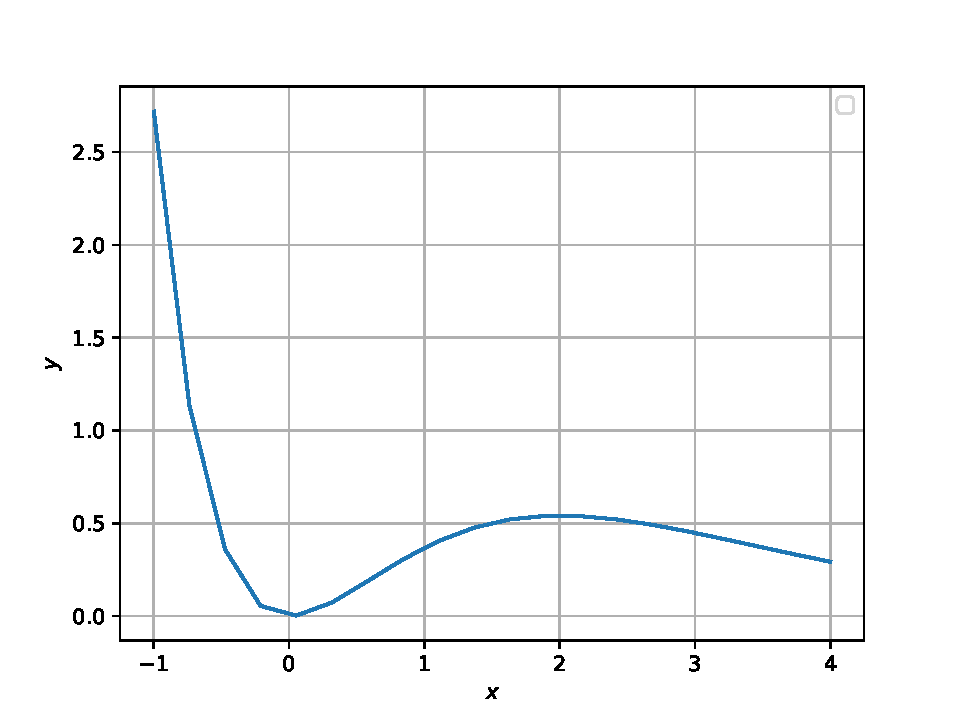
\includegraphics[width=\columnwidth]{figs/cont-12-8.pdf}
	\caption{}
	\label{fig:cont-12-8}
\end{figure}
\item The function $ f\left({x} \right) = \frac{x-1}{x\left(x^2 -1 \right)} $ is discontinuous at

\begin{enumerate}
    \item Exactly one point
    \item Exactly two points
    \item Exactly three points
    \item No point
\end{enumerate}
\solution The given function can be expressed as
		\begin{align}
			f\brak{x} = \frac{x-1}{x\brak{x-1}\brak{x+1}} 
		\end{align}
Hence, the denominator of the given function vanishes at $x = 0, 1, -1$,    
which are the points of discontinuity.  However, there is a removable discontinuity at $x = 1$.
This can be seen in Fig. 
	\ref{fig:cont-12-9},
\begin{figure}[!ht]
	\centering
	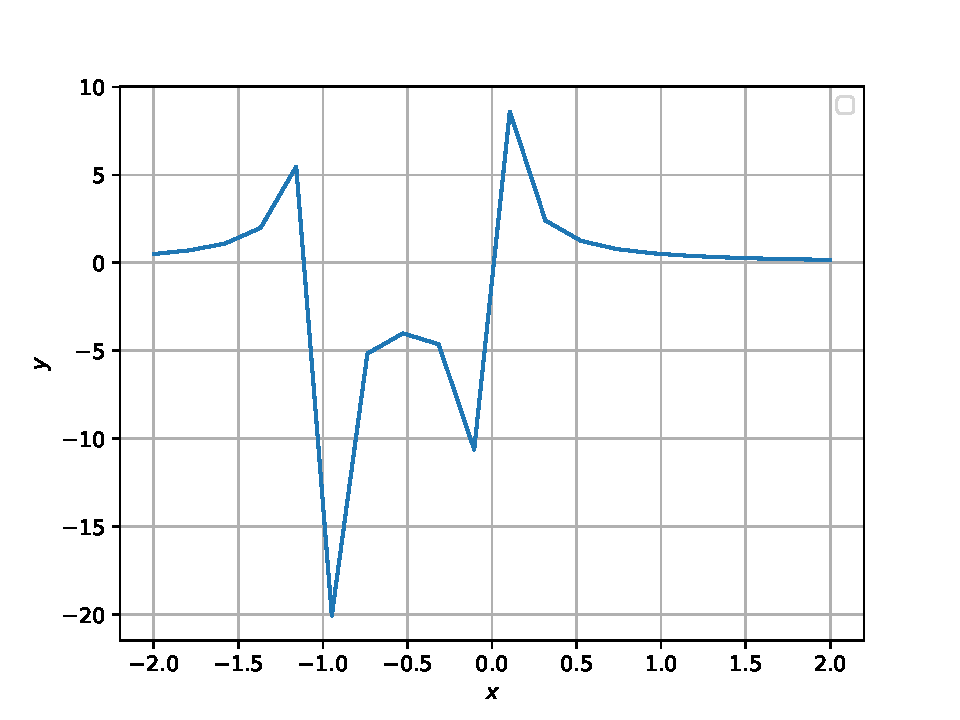
\includegraphics[width=\columnwidth]{figs/cont-12-9.pdf}
	\caption{}
	\label{fig:cont-12-9}
\end{figure}
\item The function  $ f : R \rightarrow \left[-1,1 \right] $ defined by $ f\left(x \right) = \cos x $ is

\begin{enumerate}
    \item Both one-one and onto
    \item Not one-one, but onto
    \item one-one, but Not onto
    \item Neither one-one, nor onto
\end{enumerate}
\solution 
		\begin{align}
			\cos\brak{-2\pi}
			=
			\cos\brak{2\pi} = 1
		\end{align}
		Hence, $f(x)$ is not one to one.  However, it  is onto.
This can be seen in Fig. 
	\ref{fig:cont-12-10},
\begin{figure}[!ht]
	\centering
	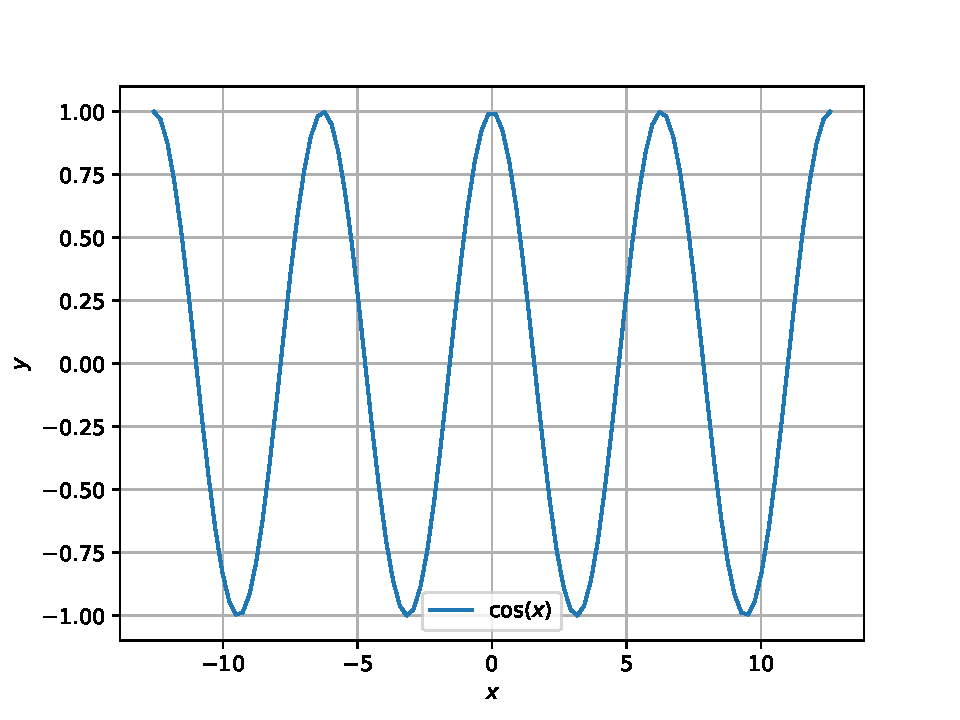
\includegraphics[width=\columnwidth]{figs/cont-12-10.pdf}
	\caption{}
	\label{fig:cont-12-10}
\end{figure}




\item  If the radius of the circle is increasing at the rate of 0.5cm/s, then the rate of increase of its circumference is ---------------\\
	\solution Let the $p$ be the circumference and $r$ the radius.  Then 
		\begin{align}
			p	&= 2\pi r
			\\
			\implies \frac{dp}{dt} &= 2\pi\frac{dr}{dt} = \pi
		\end{align}

\item \begin{enumerate} \item The range of the principle value branch of the function $ y= \sec^{-1}x $ is ----------------
			\\
			\solution The range is $\sbrak{0,\pi} - \cbrak{\frac{\pi}{2}}$.
This can be seen in Fig. 
	\ref{fig:cont-12-12},
\begin{figure}[!ht]
	\centering
	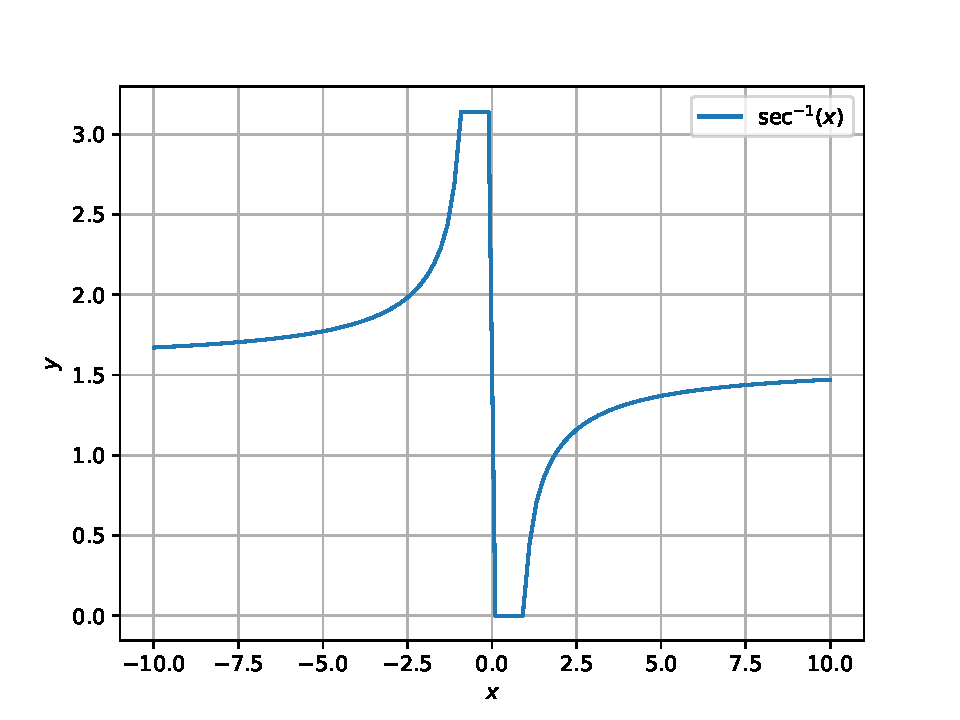
\includegraphics[width=\columnwidth]{figs/cont-12-12.pdf}
	\caption{}
	\label{fig:cont-12-12}
\end{figure}
    
\item The principal value of $\cos^{-1} \left(\frac{-1}{2}\right)$ is --------------\\
	\solution Since
		\begin{align}
			\cos \frac{\pi}{3} &= \frac{1}{2},
			\\
			\cos \brak{\pi - \frac{\pi}{3}} &= -\frac{1}{2}
		\end{align}
		Thus the desired principal value is $\frac{2\pi}{3}$
\end{enumerate}

\item  Evaluate :
	\begin{align}
         \int_{\frac{-\pi}{2}}^{\frac{\pi}{2}} x \cos^2 x dx \nonumber
	\end{align}  
	\solution $\because$ the integrand is odd, the given integral is 0. 
This can be seen in Fig. 
	\ref{fig:cont-12-13},
\begin{figure}[!ht]
	\centering
	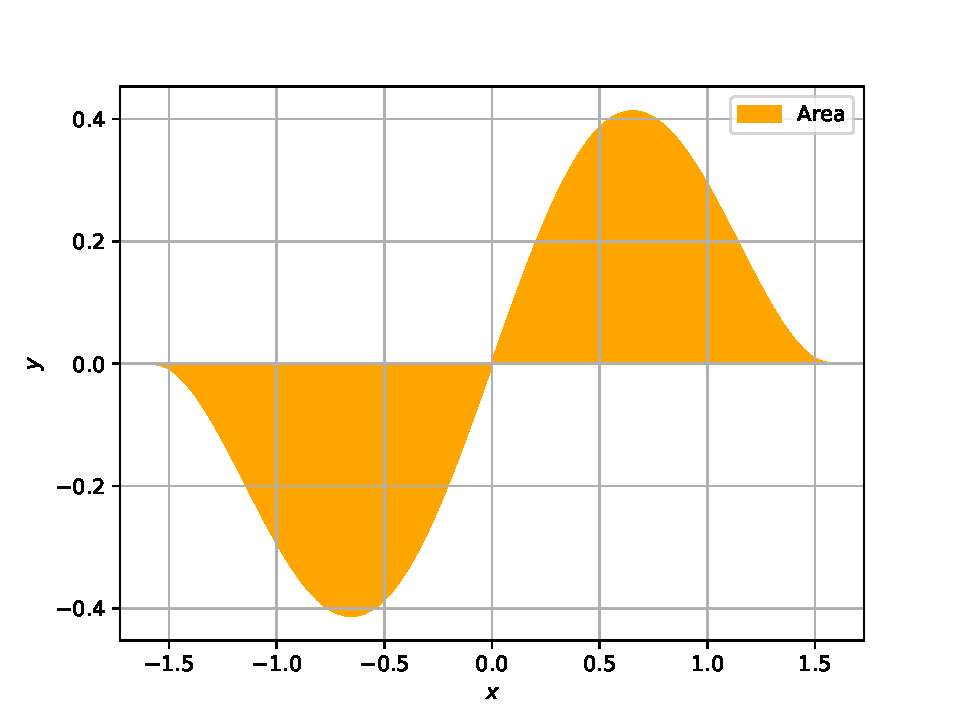
\includegraphics[width=\columnwidth]{figs/cont-12-13.pdf}
	\caption{}
	\label{fig:cont-12-13}
\end{figure}


\item  Find the value of k, so that the function 
	\begin{equation*}  f(x)  = \begin{cases}
                 k x^2 + 5,  & x \leq 1 \\
        2 , & x  >  1
\end{cases} \end{equation*} 
is continuous at x=1. \\
\solution  From the given equation, 
	\begin{align}  f(1+)  &= f(1)  
		\\
		\implies k+5 &= 2
		\\
		\text{or, } k &= -3
 \end{align} 
This can be seen in Fig. 
	\ref{fig:cont-12-14},
\begin{figure}[!ht]
	\centering
	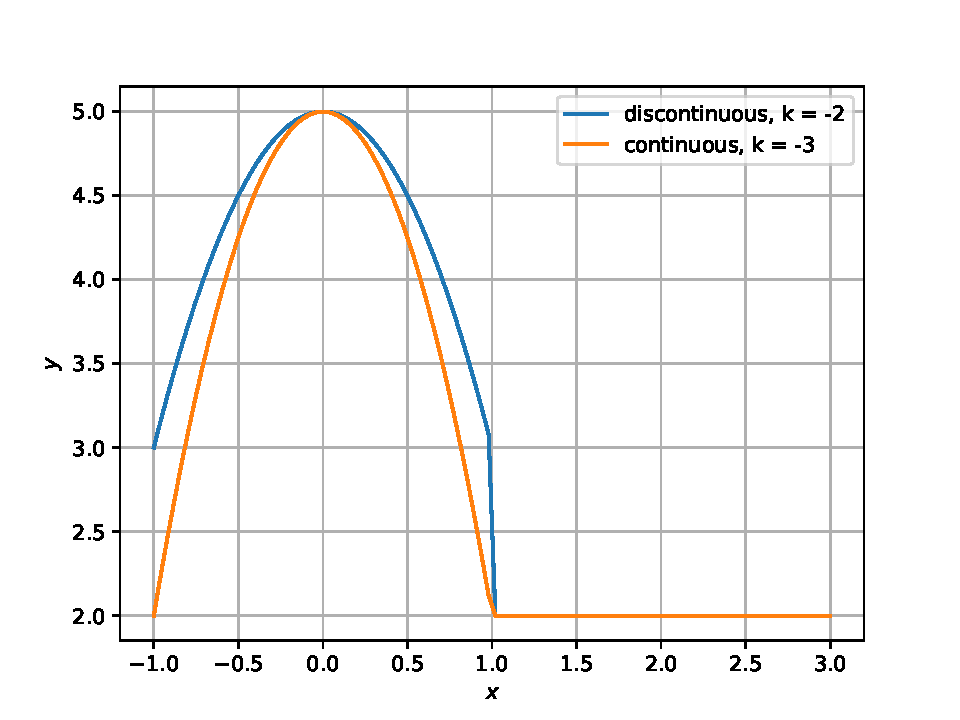
\includegraphics[width=\columnwidth]{figs/cont-12-14.pdf}
	\caption{}
	\label{fig:cont-12-14}
\end{figure}
\item  Find the integrating factor of the differential equation 
	\begin{align} 
	 x\frac{dy}{dx} = 2x^2 +y 
	\end{align} 
	\solution  The given differential equation can be expressed as
	\begin{align} 
		\frac{dy}{dx} -\frac{y}{x} = 2x 
	\end{align} 
	Letting 
	\begin{align} 
		P(x) &= -\frac{1}{x}, Q(x) = 2x,
		\\
		M(x) &= Ce^{\int P(x)\,dx} = e^{-\ln x}
		\\
		&= \frac{1}{x}
	\end{align} 
	which is the desired integrating factor.

\item If 
	\begin{align} 
		f\left(x\right)= \sqrt{\frac{\sec x-1}{\sec x+1}}\nonumber 
		\end{align} 
		Find 
		\begin{align} 
			f^{\prime}\left(\frac{\pi}{3}\right) \nonumber 
		\end{align}
		\solution The given equation can be expressed as
	\begin{align} 
		f\left(x\right)&= \sqrt{\frac{1-\cos x}{1+\cos x}}
		\\
		&=\sqrt{2 \sin^2{\frac{x}{2}}{2\cos^2 \frac{x}{2}}}
		\\
		&= \tan \frac{x}{2}
		\\
		\implies 
			f^{\prime}(x) &= f^{\prime}\brak{\frac{\pi}{3}}= \frac{1}{2}
		\end{align} 

\item Find $f^{\prime}\left(x\right)$ if 
	\begin{align} 
	f\left(x\right)=\left(\tan x\right)^{\left(\tan x\right)} 
	\end{align}
	\solution Differentiating the above, 
	\begin{multline} 
		f^{\prime}\brak{x}=\frac{d}{dx}\cbrak{\brak{\tan x}^{\brak{\tan x}} }
		\\
		=\brak{\tan x}\brak{\tan x}^{\brak{\tan x}-1}\sec^2 x
		\\
		+ \brak{\tan x}^{\brak{\tan x}} \ln \brak{\tan x}\sec^2 x
		\\
		= \sec^2\brak{\tan x}^{\brak{\tan x}}\brak{1 +\ln \brak{\tan x} }
	\end{multline}

\item Find :
	\begin{align}
		\int \frac{\tan^3x}{\cos^3x} dx 
	\end{align} 
\solution Letting 
	\begin{align}
		t = \sec x, dt &= \sec x \tan x \, dx
		\\
\implies 		\int \frac{\tan^3x}{\cos^3x} dx &= 
		\int \brak{\sec x \tan x}^3 \, dx
		\\
		&= \int t^2\brak{t^2-1}\, dt
		\\
		&= \frac{t^5}{5} - \frac{t^3}{3}
		\\
		&= \frac{\sec^5}{5} - \frac{\sec^3}{3}
	\end{align} 



\item Solve the following differential equation:
	\begin{align}
		\label{eq:diffeq}
		(1+e^{\frac{y}{x}}) dy+e^{\frac{y}{x}}\brak{1-\frac{y}{x}} dx = 0 ; (x \ne 0) 
	\end{align}
\solution  Letting
	\begin{align}
		y = xt, dy &= x\,dt + t\, dx
	\end{align}
		\eqref{eq:diffeq}
 can be expressed as
	\begin{multline}
		\brak{1+e^{t}}\brak{x\,dt + t\, dx} +e^{t}(1-t) dx = 0 
		\\
		\implies x\brak{1+e^{t}}\,dt 
		\\
		+ \cbrak{t\brak{1+e^{t}}+\brak{1-t}e^t }\,dx = 0
		\\
		\implies \frac{dx}{x} = - \frac{\brak{1+e^{t}}}{t+e^t}\,dt 
		\\
		\implies 
		\int\frac{dx}{x} = - \int\frac{\brak{1+e^{t}}}{t+e^t}\,dt 
		\\
		\text{or, }\ln x = -\ln \brak{\frac{y}{x}+e^{\frac{y}{x}}}+C_1
	\end{multline}
	Thus, 
	\begin{align}
y+xe^{\frac{y}{x}} = C
	\end{align}

\end{enumerate}
 \section{Discrete Math }
\begin{enumerate}[label=\thesection.\arabic*.,ref=\thesection.\theenumi]
\numberwithin{equation}{enumi}
\numberwithin{figure}{enumi}
\numberwithin{table}{enumi}
\item  The relation R in the set $ \{1,2,3\}$  given by $R=\{(1,2)(2,1)(1,1)\}$ is

\begin{enumerate}
    \item Symmetric and transitive, but not reflexive  \\
    \item reflexive and symmetric, but not transitive  \\
    \item Symmetric, but neither reflexive nor transitive \\
    \item An equivalence relation 
\end{enumerate}
  \item Check whether the relation R in the set N set of natural numbers given by R= \{(a,b):a is divisor of b\} is reflexive, symmetric or transitive. Also determine whether R is an equivalence relation. 
\end{enumerate}
 \section{Probability}
\begin{enumerate}[label=\thesection.\arabic*.,ref=\thesection.\theenumi]
\numberwithin{equation}{enumi}
\numberwithin{figure}{enumi}
\numberwithin{table}{enumi}
\item A card from a pack of 52 cards is lost. From the remaining cards of the pack, two cards are drawn randomly one-by-one without replacement and are found to to be both kings. Find the probability of the lost card being a king.\\
\solution See Tables 
	\eqref{table:prob-1.0}
	and 
	\eqref{table:prob-1.1}
\begin{table}[!htb]
	\input{tables/prob-1.0}
\caption{}
	\label{table:prob-1.0}
\end{table}
\begin{table}[!htb]
	\input{tables/prob-1.1}
\caption{}
	\label{table:prob-1.1}
\end{table}
for the input probabilities.
The desired probability is then obtained from 
			\eqref{eq:prob-1}
			as
			\begin{multline}
			\pr{X_1 = 1|X_2 = 1, X_3=1} 
			\\
				= \frac{\frac{1}{25}\times\frac{1}{17}\times\frac{1}{13} }{\frac{1}{25}\times\frac{1}{17}\times\frac{1}{13} +\frac{3}{50}\times\frac{4}{51}\times\frac{12}{13}   }
				= \frac{1}{25}
			\end{multline}

		\begin{figure*}[!b]
			\hrule
		\begin{multline}
			\pr{X_1 = 1|X_2 = 1, X_3=1} 
			= \frac{\pr{X_1 = 1,X_2 = 1, X_3=1}}{\pr{X_2 = 1, X_3=1}}
			\\
			= \frac{\pr{X_3 = 1 | X_1 = 1, X_2=1}\pr{X_2 = 1| X_1 = 1}\pr{X_1=1}}{\sum_{i=0}^{1}\pr{X_1 = i, X_2 = 1, X_3=1}}
			\\
			= \frac{\pr{X_3 = 1 | X_1 = 1, X_2=1}\pr{X_2 = 1| X_1 = 1}\pr{X_1=1}}{\sum_{i=0}^{1}\pr{X_3=1,| X_1 = i, X_2 = 1 }\pr{X_2 = 1| X_1 = i}\pr{X_1=i}}
			\label{eq:prob-1}
		\end{multline}
		\end{figure*}
\item A fair dice is thrown two times. Find the probability distribution of the number of sixes. Also determine the mean of the number of sixes.\\
	\solution Let $X = \cbrak{0,1,2}$ denote the sample space.  
		Table 
	\eqref{table:prob-2}
		gives the desired probability distribution.  In general, this can be expressed as a Binomial distribution with probability mass function (pmf)
		\begin{align}
			p_X(k) = \comb{n}{k}\brak{1-p}^{k}p^{n-k}, 0 \le k \le n
		\end{align}
		The mean value is then obtained as
		\begin{align}
			\mean{X} &= np = \frac{1}{3}
		\end{align}
		for $n = 2$ and $p = \frac{1}{6}$
\begin{table}[!htb]
	%%%%%%%%%%%%%%%%%%%%%%%%%%%%%%%%%%%%%%%%%%%%%%%%%%%%%%%%%%%%%%%%%%%%%%
%%                                                                  %%
%%  This is the header of a LaTeX2e file exported from Gnumeric.    %%
%%                                                                  %%
%%  This file can be compiled as it stands or included in another   %%
%%  LaTeX document. The table is based on the longtable package so  %%
%%  the longtable options (headers, footers...) can be set in the   %%
%%  preamble section below (see PRAMBLE).                           %%
%%                                                                  %%
%%  To include the file in another, the following two lines must be %%
%%  in the including file:                                          %%
%%        \def\inputGnumericTable{}                                 %%
%%  at the beginning of the file and:                               %%
%%        \input{name-of-this-file.tex}                             %%
%%  where the table is to be placed. Note also that the including   %%
%%  file must use the following packages for the table to be        %%
%%  rendered correctly:                                             %%
%%    \usepackage[latin1]{inputenc}                                 %%
%%    \usepackage{color}                                            %%
%%    \usepackage{array}                                            %%
%%    \usepackage{longtable}                                        %%
%%    \usepackage{calc}                                             %%
%%    \usepackage{multirow}                                         %%
%%    \usepackage{hhline}                                           %%
%%    \usepackage{ifthen}                                           %%
%%  optionally (for landscape tables embedded in another document): %%
%%    \usepackage{lscape}                                           %%
%%                                                                  %%
%%%%%%%%%%%%%%%%%%%%%%%%%%%%%%%%%%%%%%%%%%%%%%%%%%%%%%%%%%%%%%%%%%%%%%



%%  This section checks if we are begin input into another file or  %%
%%  the file will be compiled alone. First use a macro taken from   %%
%%  the TeXbook ex 7.7 (suggestion of Han-Wen Nienhuys).            %%
\def\ifundefined#1{\expandafter\ifx\csname#1\endcsname\relax}


%%  Check for the \def token for inputed files. If it is not        %%
%%  defined, the file will be processed as a standalone and the     %%
%%  preamble will be used.                                          %%
\ifundefined{inputGnumericTable}

%%  We must be able to close or not the document at the end.        %%
	\def\gnumericTableEnd{\end{document}}


%%%%%%%%%%%%%%%%%%%%%%%%%%%%%%%%%%%%%%%%%%%%%%%%%%%%%%%%%%%%%%%%%%%%%%
%%                                                                  %%
%%  This is the PREAMBLE. Change these values to get the right      %%
%%  paper size and other niceties.                                  %%
%%                                                                  %%
%%%%%%%%%%%%%%%%%%%%%%%%%%%%%%%%%%%%%%%%%%%%%%%%%%%%%%%%%%%%%%%%%%%%%%

	\documentclass[12pt%
			  %,landscape%
                    ]{report}
       \usepackage[latin1]{inputenc}
       \usepackage{fullpage}
       \usepackage{color}
       \usepackage{array}
       \usepackage{longtable}
       \usepackage{calc}
       \usepackage{multirow}
       \usepackage{hhline}
       \usepackage{ifthen}

	\begin{document}


%%  End of the preamble for the standalone. The next section is for %%
%%  documents which are included into other LaTeX2e files.          %%
\else

%%  We are not a stand alone document. For a regular table, we will %%
%%  have no preamble and only define the closing to mean nothing.   %%
    \def\gnumericTableEnd{}

%%  If we want landscape mode in an embedded document, comment out  %%
%%  the line above and uncomment the two below. The table will      %%
%%  begin on a new page and run in landscape mode.                  %%
%       \def\gnumericTableEnd{\end{landscape}}
%       \begin{landscape}


%%  End of the else clause for this file being \input.              %%
\fi

%%%%%%%%%%%%%%%%%%%%%%%%%%%%%%%%%%%%%%%%%%%%%%%%%%%%%%%%%%%%%%%%%%%%%%
%%                                                                  %%
%%  The rest is the gnumeric table, except for the closing          %%
%%  statement. Changes below will alter the table's appearance.     %%
%%                                                                  %%
%%%%%%%%%%%%%%%%%%%%%%%%%%%%%%%%%%%%%%%%%%%%%%%%%%%%%%%%%%%%%%%%%%%%%%

\providecommand{\gnumericmathit}[1]{#1} 
%%  Uncomment the next line if you would like your numbers to be in %%
%%  italics if they are italizised in the gnumeric table.           %%
%\renewcommand{\gnumericmathit}[1]{\mathit{#1}}
\providecommand{\gnumericPB}[1]%
{\let\gnumericTemp=\\#1\let\\=\gnumericTemp\hspace{0pt}}
 \ifundefined{gnumericTableWidthDefined}
        \newlength{\gnumericTableWidth}
        \newlength{\gnumericTableWidthComplete}
        \newlength{\gnumericMultiRowLength}
        \global\def\gnumericTableWidthDefined{}
 \fi
%% The following setting protects this code from babel shorthands.  %%
 \ifthenelse{\isundefined{\languageshorthands}}{}{\languageshorthands{english}}
%%  The default table format retains the relative column widths of  %%
%%  gnumeric. They can easily be changed to c, r or l. In that case %%
%%  you may want to comment out the next line and uncomment the one %%
%%  thereafter                                                      %%
\providecommand\gnumbox{\makebox[0pt]}
%%\providecommand\gnumbox[1][]{\makebox}

%% to adjust positions in multirow situations                       %%
\setlength{\bigstrutjot}{\jot}
\setlength{\extrarowheight}{\doublerulesep}

%%  The \setlongtables command keeps column widths the same across  %%
%%  pages. Simply comment out next line for varying column widths.  %%
\setlongtables

\setlength\gnumericTableWidth{%
	176pt+%
	151pt+%
	53pt+%
0pt}
\def\gumericNumCols{3}
\setlength\gnumericTableWidthComplete{\gnumericTableWidth+%
         \tabcolsep*\gumericNumCols*2+\arrayrulewidth*\gumericNumCols}
\ifthenelse{\lengthtest{\gnumericTableWidthComplete > \linewidth}}%
         {\def\gnumericScale{1*\ratio{\linewidth-%
                        \tabcolsep*\gumericNumCols*2-%
                        \arrayrulewidth*\gumericNumCols}%
{\gnumericTableWidth}}}%
{\def\gnumericScale{1}}

%%%%%%%%%%%%%%%%%%%%%%%%%%%%%%%%%%%%%%%%%%%%%%%%%%%%%%%%%%%%%%%%%%%%%%
%%                                                                  %%
%% The following are the widths of the various columns. We are      %%
%% defining them here because then they are easier to change.       %%
%% Depending on the cell formats we may use them more than once.    %%
%%                                                                  %%
%%%%%%%%%%%%%%%%%%%%%%%%%%%%%%%%%%%%%%%%%%%%%%%%%%%%%%%%%%%%%%%%%%%%%%

\ifthenelse{\isundefined{\gnumericColA}}{\newlength{\gnumericColA}}{}\settowidth{\gnumericColA}{\begin{tabular}{@{}p{176pt*\gnumericScale}@{}}x\end{tabular}}
\ifthenelse{\isundefined{\gnumericColB}}{\newlength{\gnumericColB}}{}\settowidth{\gnumericColB}{\begin{tabular}{@{}p{151pt*\gnumericScale}@{}}x\end{tabular}}
\ifthenelse{\isundefined{\gnumericColC}}{\newlength{\gnumericColC}}{}\settowidth{\gnumericColC}{\begin{tabular}{@{}p{53pt*\gnumericScale}@{}}x\end{tabular}}

\begin{tabular}[c]{%
	b{\gnumericColA}%
	b{\gnumericColB}%
	b{\gnumericColC}%
	}

%%%%%%%%%%%%%%%%%%%%%%%%%%%%%%%%%%%%%%%%%%%%%%%%%%%%%%%%%%%%%%%%%%%%%%
%%  The longtable options. (Caption, headers... see Goosens, p.124) %%
%	\caption{The Table Caption.}             \\	%
% \hline	% Across the top of the table.
%%  The rest of these options are table rows which are placed on    %%
%%  the first, last or every page. Use \multicolumn if you want.    %%

%%  Header for the first page.                                      %%
%	\multicolumn{3}{c}{The First Header} \\ \hline 
%	\multicolumn{1}{c}{colTag}	%Column 1
%	&\multicolumn{1}{c}{colTag}	%Column 2
%	&\multicolumn{1}{c}{colTag}	\\ \hline %Last column
%	\endfirsthead

%%  The running header definition.                                  %%
%	\hline
%	\multicolumn{3}{l}{\ldots\small\slshape continued} \\ \hline
%	\multicolumn{1}{c}{colTag}	%Column 1
%	&\multicolumn{1}{c}{colTag}	%Column 2
%	&\multicolumn{1}{c}{colTag}	\\ \hline %Last column
%	\endhead

%%  The running footer definition.                                  %%
%	\hline
%	\multicolumn{3}{r}{\small\slshape continued\ldots} \\
%	\endfoot

%%  The ending footer definition.                                   %%
%	\multicolumn{3}{c}{That's all folks} \\ \hline 
%	\endlastfoot
%%%%%%%%%%%%%%%%%%%%%%%%%%%%%%%%%%%%%%%%%%%%%%%%%%%%%%%%%%%%%%%%%%%%%%

\hhline{|-|-~}
	 \multicolumn{1}{|p{\gnumericColA}|}%
	{\gnumericPB{\centering}\gnumbox{\textbf{Probability}}}
	&\multicolumn{1}{p{\gnumericColB}|}%
	{\gnumericPB{\centering}\gnumbox{\textbf{Value}}}
	&
\\
\hhline{|--|~}
	 \multicolumn{1}{|p{\gnumericColA}|}%
	{\gnumericPB{\centering}\gnumbox{$\pr{X = 0}$ }}
	&\multicolumn{1}{p{\gnumericColB}|}%
	{\gnumericPB{\centering}\gnumbox{$\frac{5}{6}\times \frac{5}{6} = \frac{25}{36}$}}
	&
\\
\hhline{|--|~}
	 \multicolumn{1}{|p{\gnumericColA}|}%
	{\gnumericPB{\centering}\gnumbox{$\pr{X = 1}$ }}
	&\multicolumn{1}{p{\gnumericColB}|}%
	{\gnumericPB{\centering}\gnumbox{$2 \times \frac{5}{6}\times \frac{1}{6} = \frac{5}{18}$}}
	&
\\
\hhline{|--|~}
	 \multicolumn{1}{|p{\gnumericColA}|}%
	{\gnumericPB{\centering}\gnumbox{$\pr{X=2}$ }}
	&\multicolumn{1}{p{\gnumericColB}|}%
	{\gnumericPB{\centering}\gnumbox{$\frac{1}{6}\times \frac{1}{6} = \frac{1}{36}$}}
	&
	\\
\hhline{|-|-|~}
\end{tabular}

\ifthenelse{\isundefined{\languageshorthands}}{}{\languageshorthands{\languagename}}
\gnumericTableEnd

\caption{}
	\label{table:prob-2}
\end{table}
\end{enumerate}
 \section{Linear Programming}
\begin{enumerate}[label=\thesection.\arabic*.,ref=\thesection.\theenumi]
\numberwithin{equation}{enumi}
\numberwithin{figure}{enumi}
\numberwithin{table}{enumi}
\item  The corner points of the feasible region of an LPP are (0,0),(0,8),(2,7),(5,4) and (6,0). The maximum profit P=3x+2y occurs at the point .................\\
	\solution The profit can be expressed as
\begin{align}
	P=\myvec{3  & 2} \vec{x}
    \end{align}
    and the respective values at each of the above points are given by 
\begin{align}
	\myvec{3  & 2}\myvec{0\\0} &= 0,
	\\
	\myvec{3  & 2}\myvec{0\\8} & = 16
	\\
	\myvec{3  & 2}\myvec{2\\7} &= 20
	\\
	\myvec{3  & 2}\myvec{5\\4} &= 23
	\\
	\myvec{3  & 2} \myvec{6\\0} &= 18 
    \end{align}
    Hence, the maximum profit is $P = 23$ which occurs at $\myvec{5\\4}$
\item A cottage industry manufactures pedestal lamps and wooden shades. Both the products require machine time as well as craftsman time in the making. The number of hours required for producing 1 unit of each and the corresponding profit is given in the following table :
\begin{table}[htb]
\tiny
%\begin{center}
\resizebox{\columnwidth}{!}{
\begin{tabular}{|c|c|c|c|}
\hline
% \begin{tabularx}{\linewidth} {lX}
 Item & Machine Time & Craftsman Time & Profit(in INR) \\ 
 \hline
 Pedestal Lamp & 1.5 hours & 3 hours & 30\\  
 \hline
 Wooden shades & 3 hours & 1 hour & 20 \\
 \hline
%  \end{tabularx}
\end{tabular}
}
\caption{}
\end{table}
%\end{center}
In a day, the factory has availability of not more than 42 hours of machine time and 24 hours of craftsman time.\\
Assuming that all items manufactured are sold, how should the manufacturer schedule his daily production in order to maximise the profit? Formulate it as an LPP and solve it graphically.\\
\solution Let $x$ be the number of lamps and $y$ be the number of wooden shades produced.  From the given information, the problem can be formulated as
\begin{align}
	P = \max_{x,y}30x+20y
	\\
1.5x+3y \le 42
\\
3x+y \le 24
\end{align}
which can be expressed in vector form as
\begin{align}
	P = \max_{\vec{x}}\myvec{30 &20}\vec{x}
	\\
	\myvec{1 &2 \\ 3 & 1} \vec{x}\preceq \myvec{28 \\ 24}
	\\
	\vec{x} \succeq \vec{0}
\end{align}
		\begin{enumerate}
			\item {\em Graphical solution:} 

From Fig. 
	\ref{fig:opt-12-2},
\begin{figure}[!h]
	\centering
	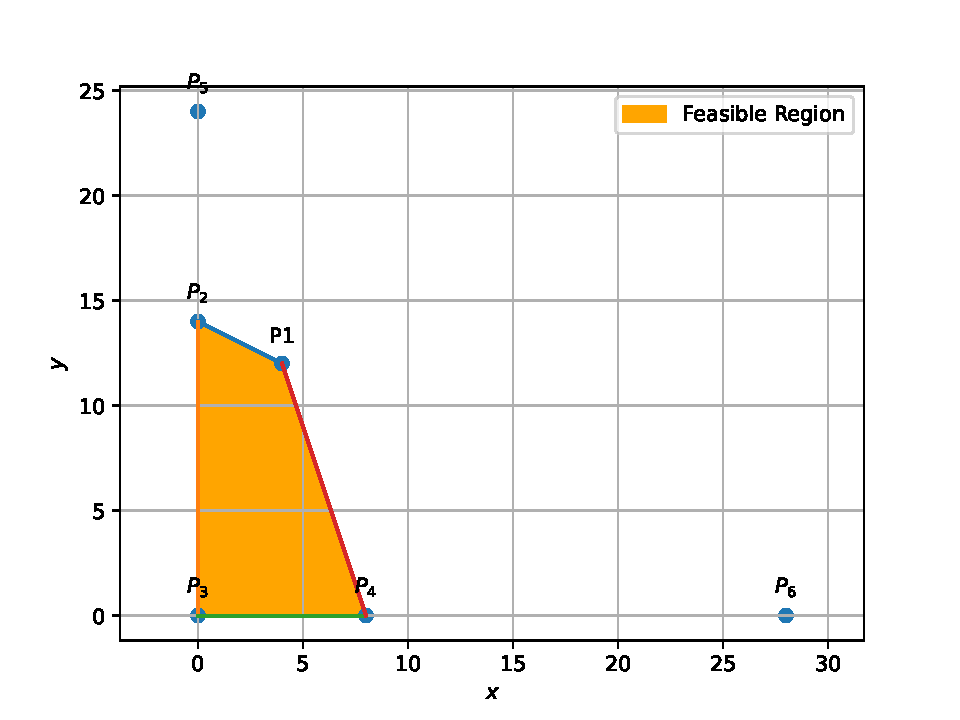
\includegraphics[width=\columnwidth]{figs/opt-12-2.pdf}
	\caption{}
	\label{fig:opt-12-2}
\end{figure}
				the feasible region is a quadrilateral with vertices
\begin{align}
\myvec{0 \\ 0},
\myvec{8 \\ 0},
\myvec{0 \\ 14},
\myvec{4 \\ 12}
\end{align}
with respective profit
\begin{align}
	\myvec{30 &20}\myvec{0 \\ 0} &= 0 \\
	\myvec{30 &20}\myvec{8 \\ 0} &= 240 \\
	\myvec{30 &20}\myvec{0 \\ 14} &= 280 \\
	\myvec{30 &20}\myvec{4 \\ 12} &= 360
\end{align}
Thus, the manufacturer should produce 4 pedestal lamps and 12 wooden shades daily.
\item {\em Lagrange Multipliers: } The given problem is expressed in the form 
\begin{align}
	P = -\min_{\vec{x}}\myvec{30 &20}\vec{x}
	\\
	\myvec{1 &2 \\ 3 & 1 \\ -1 & 0 \\ 0 & -1} \vec{x}\preceq \myvec{28 \\ 24 \\0 \\ 0}
\end{align}

	The Lagrangian, defined as the linear combination of the loss function and the constraints is defined as
	\begin{multline}
		L\brak{\vec{x},\bm{\lambda}} =-\myvec{30 & 20}\vec{x} 
		\\
		+ \lambda_1\sbrak{\myvec{1 & 2}\vec{x}-28}
		\\
		+
\lambda_2\sbrak{\myvec{3 & 1}\vec{x}-24}+
\lambda_3\sbrak{\myvec{-1 & 0}\vec{x}}
\\
+
\lambda_4\sbrak{\myvec{0 & -1}\vec{x}}
	\end{multline}
	Taking the derivative
				\begin{align}
					{\nabla L\brak{\vec{x},\bm{\lambda}}} = 0,
				\end{align}
				we obtain 
				\begin{align}
					 \lambda_1 + 3\lambda_2 -\lambda_3 &= 30
					\\
					 2\lambda_1 + \lambda_2 -\lambda_4 &= 20
					\\
					x_1 + 2x_2 &= 28
					\\
					3x_1 + x_2 &= 24
					\\
					x_1  &= 0
					\\
					x_2 &= 0
				\end{align}
				It is obvious that $x_1=0, x_2=0$ are infeasible.  Hence, considering only $\lambda_1, \lambda_2$ as the active multipliers, the above equations can be expressed as
				\begin{align}
					\myvec{0 & 0 &1 & 3 
\\
					0 & 0 & 2 & 1
					\\
					1 & 2 & 0 & 0
					\\
					3 & 1 & 0 & 0
					}
					\myvec{\vec{x} \\ \bm{\lambda}} = \myvec{30\\20\\28\\24}
					\end{align}
					yielding the optimal solution as
					\begin{align}
						\myvec{\vec{x} \\ \bm{\lambda}} = \myvec{4\\12\\6\\8}
					\end{align}
		\end{enumerate}
 \item Amongst all open (from the top) right circular cylindrical boxes of volume $125 \pi $ $cm^3$, find the dimensions of the box which has the least surface area.\\  
\solution Let $r$ be the radius of the cylinder and $h$ be the height.  Then the surface area is 
		\begin{align}
			\label{eq:opt-box-S}
			S &= \pi r^2 + 2\pi r h 
		\end{align}
		Also, the volume is 
		\begin{align}
			\label{eq:opt-box-V}
			V &= \pi r^2 h 
		\end{align}
		\begin{enumerate}
			\item 
		The given problem can then be formulated as 
		\begin{align}
			S = \min_{r,h}\pi r^2 + 2\pi r h 
			\\
			\text{s.t} \quad \pi r^2 h =125 
		\end{align}
				which is a {\em disciplined geometric programming} (DGP) problem that can be solved using $cvxpy$. DGP is a subset of 
				 {\em log-log-convex program} (LLCP). An LLCP is defined as

				\begin{equation}
\begin{split}
\begin{array}{ll}
\mbox{minimize} & f_0(x) \\
\mbox{subject to} & f_i(x) \leq \tilde{f_i}, \quad i=1, \ldots, m\\
& g_i(x) = \tilde{g_i}, \quad i=1, \ldots, p,
\end{array}
\end{split}
\end{equation}

where the functions $f_i$
				are log-log convex, $\tilde{f}_i$
 are log-log concave, and the functions $g_i$
				and $\tilde{g}_i$
 are log-log affine. An optimization problem with constraints of the above form in which the goal is to maximize a log-log concave function is also an LLCP.
A function 
				\begin{align}
 f : D \subseteq \mathbf{R}^{n}_{++} \to \mathbf{R}
				\end{align}
				is said to be log-log convex if the function
				\begin{align}
				F(u)=\log f(e^u)
				\end{align}
				with domain
				\begin{align}
				\{u \in \mathbf{R}^n : e^u \in D\}
				\end{align}
				is convex (where
$				\mathbf{R}^{n}_{++}$
				denotes the set of positive reals and the logarithm and exponential are meant elementwise); the function $F$  is called the log-log transformation of $f$. The function $f$ is log-log concave if $F$ is concave, and it is log-log affine if $F$ is affine.
				LLCPs are problems that become convex after the variables, objective functions, and constraint functions are replaced with their logs, an operation that we refer to as a log-log transformation. LLCPs generalize geometric programming.

	\item 
		Alternatively, from 
			\eqref{eq:opt-box-S} and 
			\eqref{eq:opt-box-V}
		\begin{align}
			S(r) &= \pi r^2 +  \frac{2 V}{r} 
			\\
			\label{eq:opt-box-Sdiff}
			\implies 
			S^{\prime}(r) &= 2\pi r -  \frac{2 V}{r^2} 
			\\
			\text{and }
			S^{\prime\prime}(r) &= 2\pi  +  \frac{4 V}{r^3} > 0 
		\end{align}
		Thus, $S(r)$ has a minimum which can be obtained from 
			\eqref{eq:opt-box-Sdiff} as
		\begin{align}
			2\pi r -  \frac{2 V}{r^2} &= 0
			\\
			\implies r &= \brak{\frac{V}{\pi}}^{\frac{1}{3}}
			\\
			&= 5 \quad \text{and }
			\\
			h &= \frac{V}{\pi r^2} = 5
		\end{align}
		upon substituting numerical values.
		This is verified in 
Fig. 
	\ref{fig:opt-12-3}.
\begin{figure}[!h]
	\centering
	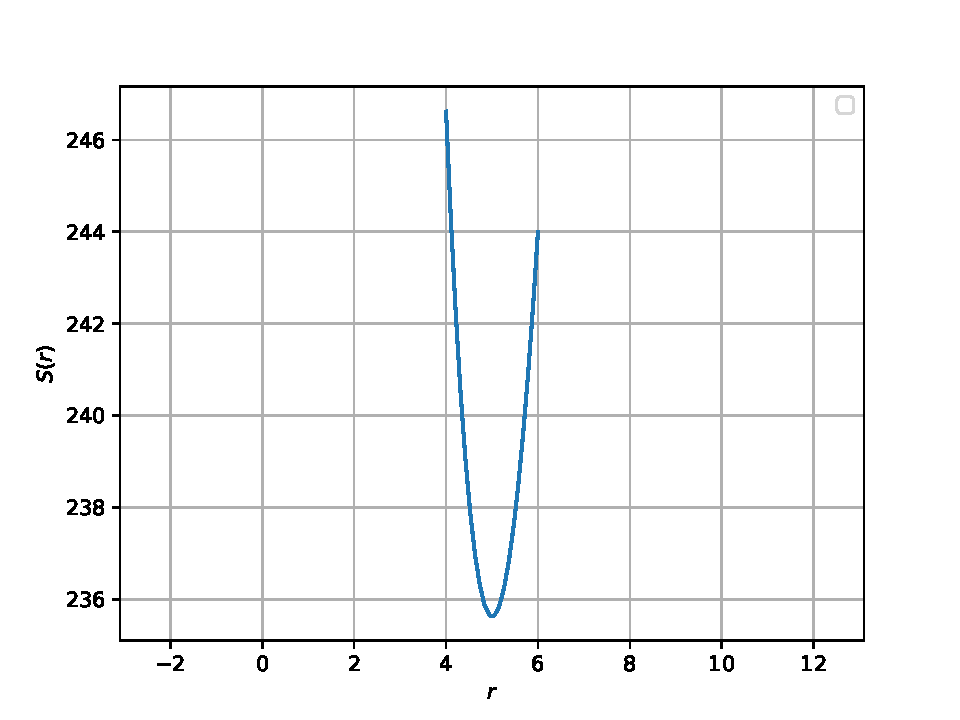
\includegraphics[width=\columnwidth]{figs/opt-12-3.pdf}
	\caption{}
	\label{fig:opt-12-3}
\end{figure}
	\item Using gradient descent, the update equation can be expressed as 
		\begin{align}
			r_{n+1} &= r_n - \gamma S^{\prime}(r_n)
		\end{align}
		where $r_0 = 2$ and $\gamma = 0.001$ are chosen by the user.  These values need to be suitably guessed for the algorithm to converge.


\end{enumerate}
\end{enumerate}
\end{document}
